\subsection{Trojhladinový systém}
    Uvažujte jednoduchý trojhladinový systém, kde index hladiny je $h=1,2,3$, první hladina má energii $d$ a vzdálenost mezi sousedními hladinami je také $d$ (jednočásticové spektrum je ekvidistantní).
    Na každé hladině se můžou nacházet nanejvýš dvě částice (každá hladina je dvojnásobně degenerovaná).
    Jednočásticové stavové vektory jsou $\ket{h\sigma}$, kde $\sigma=\pm$.

	\begin{figure}[!htbp]
        \centering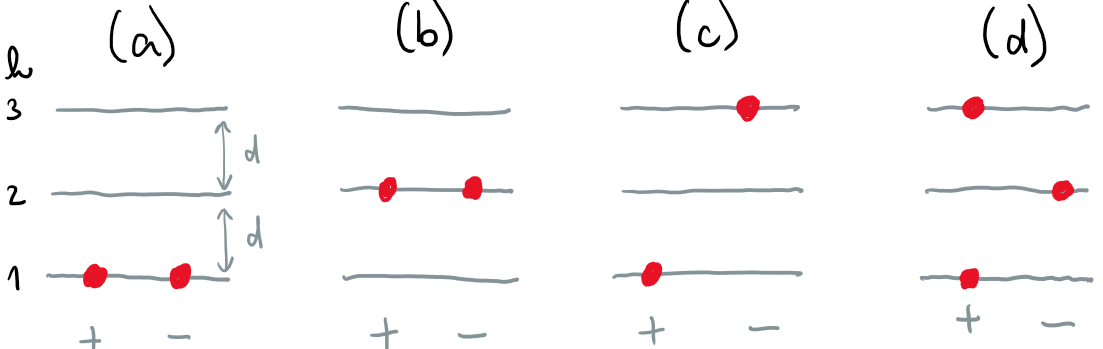
\epsfig{file=3levels.png,width=0.7\linewidth}
		\caption{
			Příklady několika možných vícečásticových konfigurací v trojhladinovém systému.
		}
    \label{fig:ThreeLevel}
	\end{figure}				

    \begin{enumerate}
        \item Kolik odlišných dvoučásticových stavových vektorů (Slaterových determinantů) lze zkonstruovat? 
        
        \item Předpokládejte, že v systému jsou pouze dvě částice, které se mohou nacházet výhradně v páru na jedné z nejnižších dvou hladin $h=1$ a $h=2$ [obrázek~\ref{fig:ThreeLevel}~(a)--(b)] a že jeho Hamiltonián má tvar
        \begin{equation}
            \operator{H}=\operator{H}_{0}+\operator{H}_{\mathrm{I}},
        \end{equation}
        přičemž jednočásticová část Hamiltoniánu splňuje
        \begin{equation}
            \operator{h}_{0}\ket{h\sigma}=hd\ket{h\sigma}.
        \end{equation}
        Dvoučásticové maticové elementy Hamiltoniánu $\operator{H}_{\mathrm{I}}$ mají všechny stejnou hodnotu $g$.
        Jak vypadá matice Hamiltoniánu $\operator{H}$?

        \item
            Jaké jsou vlastní hodnoty a vlastní vektory matice $\matrix{H}$?

        \item
            Jaký je překryv stavu odpovídajícího nižšímu vlastnímu stavu Hamiltoniánu $\operator{H}$ s dvoučásticovým stavem popisujícím dvě částice na hladině $p=2$?\footnote{
                Někdy se také říká, že se jedná o \emph{příměs} stavu $\ket{\psi_{2}}$ k základnímu stavu.
            }
            
        \item
            Přidejte nyní třetí hladinu, přičemž předpokládejte stále, že se částice mohou nacházet pouze v párech.
    \end{enumerate}

    \begin{solution}
        \begin{enumerate}
            \item Počty vícečásticových stavů lze určit obecně pro systém $n$ částic s $H$ hladinami.
                Celkový počet pozic, na které můžeme částice umístit, je $P=2H$ (počet hladin krát počet částic, které lze umístit na jednu hladinu).
                Počet $n$-částicových funkcí je pak dán počtem všech možných kombinací $n$ částic na $P$ pozicích, tj.
                \begin{equation}
                    N=\makematrix{2H \\ n}.
                \end{equation}

                Konkrétně pro $H=3$ a $n=2$ vychází
                \begin{equation}
                    N=15.
                \end{equation}
                Všechny 15 možných konfigurací je znázorněno na obrázku~\ref{fig:ThreeLevelTwoParticles}.

                \begin{figure}[!htbp]
                    \centering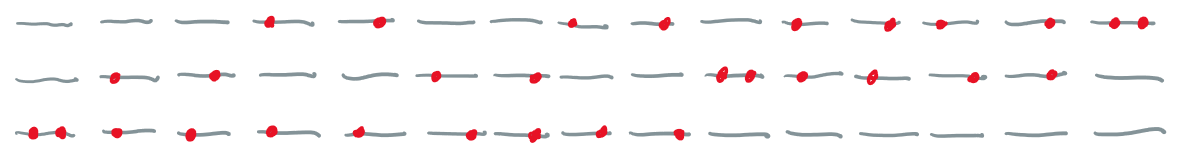
\epsfig{file=3levels2particles.png,width=0.9\linewidth}
                    \scaption{
                        Všechny možné dvoučásticové konfigurace v tříhladinovém systému.
                    }
                    \label{fig:ThreeLevelTwoParticles}
                \end{figure}				
            
            \item
                Podprostor uvažovaných dvoučásticových stavů ($n=2$) je dvourozměrný a stavy jsou dány Slaterovými determinanty\sfootnote{
                    Zkrácený zápis je nutné číst jako
                    \begin{equation}
                        \ket{1+}\ket{1-}\equiv\ket{1+}^{(1)}\otimes\ket{1-}^{(2)},
                    \end{equation}
                    tj. první ket odpovídá první částici, druhý ket druhé částici.
                }
                \begin{equation}
                    \label{eq:ThreeLevelTwoPairs}
                    \ket{\psi_{j}}=\frac{1}{\sqrt{n!}}\det{\makematrix{\ket{j+} & \ket{j+} \\ \ket{j-} & \ket{j-}}}\Rightarrow
                    \begin{cases}
                        \ket{\psi_{1}}=\frac{1}{\sqrt{2}}\left(\ket{1+}\ket{1-}-\ket{1-}\ket{1+}\right),\\
                        \ket{\psi_{2}}=\frac{1}{\sqrt{2}}\left(\ket{2+}\ket{2-}-\ket{2-}\ket{2+}\right).
                    \end{cases}
                \end{equation}
                Tyto stavy jsou normalizované a na sebe kolmé.

                Dvoučásticový volný Hamiltonián je
                \begin{equation}
                    \operator{H}_{0}=\operator{h}_{0}^{(1)}+\operator{h}_{0}^{(2)}=\operator{h}_{0}\otimes\operator{1}+\operator{1}\otimes\operator{h}_{0}
                \end{equation}
                a pro jeho maticové elementy v bázi dané vektory~\eqref{eq:ThreeLevelTwoPairs} platí
                \begin{align}
                    \matrixelement{\psi_{j}}{\operator{H}_{0}}{\psi_{k}}
                        &=\frac{1}{2}\left(\bra{j+}\bra{j-}-\bra{j-}\bra{j+}\right)\operator{H}_{0}\left(\ket{k+}\ket{k-}-\ket{k-}\ket{k+}\right)\nonumber\\
                        &=\frac{1}{2}\bigg(\underbrace{\matrixelement{j+}{\operator{h}_{0}}{k+}}_{jd\delta_{jk}}\underbrace{\braket{j-}{k-}}_{\delta_{jk}}
                            +\underbrace{\braket{j+}{k+}}_{\delta_{jk}}\underbrace{\matrixelement{j-}{\operator{h}_{0}}{k-}}_{jd\delta_{jk}}\nonumber\\
                        &\quad\ \ \underbrace{-\matrixelement{j+}{\operator{h}_{0}}{k-}}_{0}\underbrace{\braket{j-}{k+}}_{0}
                            -\underbrace{\braket{j+}{k-}}_{0\dotsb}\matrixelement{j-}{\operator{h}_{0}}{k+}\nonumber\\
                        &\quad\ \ -\matrixelement{j-}{\operator{h}_{0}}{k+}\braket{j+}{k-}
                            -\braket{j-}{k+}\matrixelement{j+}{\operator{h}_{0}}{k-}\nonumber\\
                        &\quad\ \ +\matrixelement{j-}{\operator{h}_{0}}{k-}\braket{j+}{k+}
                            +\braket{j-}{k-}\matrixelement{j+}{\operator{h}_{0}}{k+}\bigg)\nonumber\\
                        &=\frac{1}{2}\left(jd+jd+jd+jd\right)\delta_{jk}=2jd\delta_{jk},
                \end{align}
                což v maticové realizaci dá
                \begin{equation}
                    \matrix{H}_{0}=\makematrix{2d & 0 \\ 0 & 4d}.
                \end{equation}
                Matice interakčního Hamiltoniánu má tvar
                \begin{equation}
                    \matrix{H}_{\mathrm{I}}=\makematrix{g & g \\ g & g},
                \end{equation}
                takže celkový Hamiltonián je
                \begin{equation}
                    \label{eq:ThreeLevelH}
                    \matrix{H}=\makematrix{2d + g & g \\ g & 4d + g}.
                \end{equation}

            \item
                Matici~\eqref{eq:ThreeLevelH} lze přepsat na tvar
                \begin{equation}
                    \matrix{H}=\left(3d+g\right)\matrix{1}-d\sigma_{3}+g\sigma_{1},
                \end{equation}
                čož odpovídá Hamiltoniánu detailně propočteném v příkladu~\ref{sec:AvoidedCrossing}, kde se přiřadí $d\leftrightarrow e,g\leftrightarrow\nu$, výsledné spektrum se posune v energii o $3d+g$ a prohodí se vlastní vektory.
                Vlastní hodnoty jsou tedy
                \begin{equation}
                    E_{\pm}=3d+g\pm\sqrt{d^{2}+g^{2}}
                \end{equation}
                a odpovídající vlastní vektory
                \begin{subequations}
                    \begin{align}
                        \ket{\phi_{-}}&=\alpha\ket{\psi_{2}}+\beta\ket{\psi_{1}},\\
                        \ket{\phi_{+}}&=\beta\ket{\psi_{2}}-\alpha\ket{\psi_{1}},
                    \end{align}                        
                \end{subequations}
                kde koeficienty $\alpha$ a $\beta$ jsou dány vztahy~\eqref{eq:TwoLevelEV}.
                Vektory $\ket{\phi_{\pm}}$ jsou jen lineární kombinací vektorů antisymetrických vůči záměně částic, samy jsou tedy antisymetrické při záměně $\ket{j\sigma}^{(1)}\leftrightarrow\ket{j\sigma}^{(2)}$.

            \item
                Překryv je dán amplitudou pravděpodobnosti
                \begin{equation}
                    \braket{\psi_{2}}{\phi_{-}}=\alpha=\frac{g}{\sqrt{g^{2}+\left(d+\sqrt{g^{2}+d^{2}}\right)}}\sim\frac{1}{2}\frac{g}{e},
                \end{equation}
                kde poslední rovnost platí pro $g\ll e$.

            \item
                Rozšíření systému o třetí hladinu vede na matici Hamiltoniánu
                \begin{equation}
                    \matrix{H}'=\makematrix{2d + g & g & g \\ g & 4d + g & g \\ g & g & 6d + g},
                \end{equation}
                kterou je nutné řešit numericky pro konkrétní hodnoty parametrů $d,g$.
            \end{enumerate}
    \end{solution}

    \begin{note}
        Dodatečné kvantové číslo jednočásticových stavů označené $\sigma$ lze identifikovat s projekcí spinu částice.
        Pak je možné rozdělit Hilbertův prostor jednočásticových stavů jako $\hilbert{H}_{1}=\hilbert{H}_{1\mathrm{h}}\otimes\hilbert{H}_{1\mathrm{p}}$, kde první odpovídá umístění částice na jednu z hladin a druhý pak jejímu spinu.

        Dvoučásticový Hilbertův prostor lze pak rozdělit na
        \begin{equation}
            \hilbert{H}_{2}=\left(\hilbert{H}_{2\mathrm{h}}^{\mathrm{S}}\otimes\hilbert{H}_{2\mathrm{s}}^{\mathrm{S}}\right)\oplus\left(\hilbert{H}_{2\mathrm{h}}^{\mathrm{A}}\otimes\hilbert{H}_{2\mathrm{s}}^{\mathrm{T}}\right),
        \end{equation}
        kde $\hilbert{H}_{2\mathrm{h}}^{S,A}$ je symetrická, resp. antisymetrická kombinace hladinových stavů a $\hilbert{H}_{2\mathrm{s}}^{S,T}$ je singletní, resp. tripletní spinový stav.
        Stavy~\eqref{eq:ThreeLevelTwoPairs} pak mají symetrickou hladinovou a singletní (antisymetrickou) spinovou část,
        \begin{equation}
            \ket{\psi_{j}}=\ket{jj}\otimes\ket{00},
        \end{equation}
        kde
        \begin{subequations}            
            \begin{equation}
                \ket{jj}=\ket{j}^{(1)}\otimes\ket{j}^{(2)}
            \end{equation}
            je hladinová část a
            \begin{equation}
                \ket{00}=\frac{1}{\sqrt{2}}\left(\ket{+}^{(1)}\otimes\ket{-}^{(2)}-\ket{-}^{(1)}\otimes\ket{+}^{(2)}\right)
            \end{equation}
            je singletní spinový stav.
        \end{subequations}
    \end{note}

    \begin{note}
        Se singletními a tripletními spinovými stavy se také počítá v příkladech~\ref{sec:Mionium}, \ref{sec:VanDerWaals} a~\ref{sec:GaussovskaPoruchaFermiony}.
    \end{note}